\newcommand{\defs}{../defs}
\documentclass[12pt,oneside,chapterprefix=true]{scrbook}

\usepackage[T1]{fontenc}
\usepackage[utf8x]{inputenc}
\usepackage[brazilian]{babel}
\usepackage[table]{xcolor}
\usepackage{minted}
\usepackage[a5paper,left=0.7cm,right=0.7cm,top=2cm,bottom=2.5cm,]{geometry}
\usepackage{url}
\usepackage{graphicx}
\usepackage[export]{adjustbox}
\usepackage{hyperref}
\usepackage[square]{natbib}
\usepackage[parfill]{parskip}
\usepackage{mdframed}
\usepackage{longtable}
\usepackage{soul}
\usepackage{tabularx}
\usepackage[shortlabels]{enumitem}
\usepackage{xifthen}
\usepackage{multirow}
\usepackage[portuguese, ruled, vlined, linesnumbered, algochapter]{algorithm2e}
\usepackage{amsmath}
\usepackage{amssymb}
\usepackage{amsthm}
\usepackage{tablefootnote}
\usepackage{subfigure}
\usepackage{gensymb}
\usepackage{pgfplots}
\usepackage{xpatch}
\usepackage{varwidth}
\usepackage[htt]{hyphenat}

\renewcommand{\familydefault}{\sfdefault}

\newcommand{\name}{Prof. Marcelo de Souza}
\newcommand{\email}{marcelo.desouza@udesc.br}
\newcommand{\course}{Bacharelado em Engenharia de Software}
\newcommand{\university}{Universidade do Estado de Santa Catarina}
\newcommand{\campus}{Centro de Educação Superior do Alto Vale do Itajaí}
\newcommand{\shortuniversity}{UDESC Ibirama}
\newcommand{\version}{Versão compilada em \today}
\newcommand{\exercisedescription}{Exercício}

\usepackage[automark,headsepline,footsepline]{scrlayer-scrpage}
\lehead{\content}
\lohead{\content}
\rehead{}
\rohead{}
\cehead{}
\cohead{}
\lefoot{\name}
\lofoot{\name}
\refoot{\\\thepage}
\rofoot{\\\thepage}
\cofoot{}
\cefoot{}
\setkomafont{pagehead}{\normalfont\small}
\setkomafont{pagefoot}{\normalfont}

\newpairofpagestyles{firstpage}{}

\newcommand{\makeheader}{
	\thispagestyle{firstpage}
	\vspace*{-42pt}
	\framebox[\textwidth]{
		\parbox{0.97\textwidth}{
			\begin{center}
				{\scriptsize\shortcourse\ -- \class}
				
				\vspace{10pt}
				
				\textbf{\content}
				
				\vspace{2pt}
				
				{\small\name}
				
				\vspace{10pt}
				
				{\scriptsize\shortuniversity\hfill\email}
				
				\vspace{-5pt}
				
				{\scriptsize\course\hfill\version}
				
			\end{center}
		}
	}
%	\vspace{-15pt}
%	\begin{flushright}
%		{\scriptsize\source}
%	\end{flushright}
	\smallskip
}

\renewcommand{\thesection}{\arabic{section}}

\allowdisplaybreaks

\hypersetup{
	colorlinks,
	linkcolor={blue!80!black},
	citecolor={blue!80!black},
	urlcolor={blue!80!black}
}

\definecolor{codelinecolor}{gray}{.90}
\colorlet{codeboxcolor}{blue!8}

\surroundwithmdframed{minted}

\BeforeBeginEnvironment{mdframed}{}
\AfterEndEnvironment{mdframed}{}

\mdfsetup{%
	backgroundcolor=codeboxcolor,
	linecolor=white}

\setminted{%
	mathescape,
	escapeinside=@@,
	linenos,
	breaklines,
	tabsize=3,
	fontsize=\footnotesize}

\newcommand{\code}[1]{%
	\sethlcolor{codelinecolor}
	\texttt{\hl{#1}}%
}

\newcommand{\inblock}[1]{%
	\sethlcolor{blockcolor}
	\hl{\mbox{#1}}%
}

\newcommand{\javacode}[1]{%
	\mintinline[escapeinside=~~]{java}{#1}
}

\newcommand{\javacodecolor}[1]{%
	\mintinline[escapeinside=~~,bgcolor=codeboxcolor]{java}{#1}
}

\newcounter{number}
\newenvironment{exercise}[1][]
{%
	\refstepcounter{number}%
	\noindent%
	\ifthenelse{\equal{#1}{}}%
		{\textbf{\exercisedescription~\thenumber.\\}}%
		{\textbf{\exercisedescription~\thenumber. (#1)\\}}%
	\rmfamily%
}{\medskip}%

\newcommand{\resetexercisenumbering}{
	\setcounter{number}{0}
}

\newcounter{solutionnumber}
\newenvironment{solution}[1][]
{%
	\refstepcounter{solutionnumber}%
	\noindent%
	\ifthenelse{\equal{#1}{}}%
	{\textbf{Solução -- \exercisedescription~\thesolutionnumber.\\}}%
	{\textbf{Solução -- \exercisedescription~\thesolutionnumber. (#1)\\}}%
	\rmfamily%
}{\medskip}%

\makeatletter%
\setlength{\@fptop}{5pt}

\def\arraystretch{1.5}

\newcommand{\insertspace}{\vspace{1.2em}}
\newcommand{\removespace}{\vspace{-1.2em}}

\setlength{\fboxsep}{0.8em}

\usepackage{array}
\newcolumntype{L}[1]{>{\raggedright\let\newline\\\arraybackslash\hspace{0pt}}m{#1}}
\newcolumntype{C}[1]{>{\centering\let\newline\\\arraybackslash\hspace{0pt}}m{#1}}
\newcolumntype{R}[1]{>{\raggedleft\let\newline\\\arraybackslash\hspace{0pt}}m{#1}}

\colorlet{blockcolor}{red!25}
\colorlet{redtext}{red!60!black}

\newcommand{\block}[1]{%
	\medskip
	\begin{figure}[H]
		\centering
		\begin{tikzpicture}
		\node [rectangle, align=center, fill=blockcolor, rounded corners=0.04cm, opacity = 1, text opacity = 1] {%
			#1
		};
		\end{tikzpicture}
	\end{figure}
}

\newcommand{\newtitle}[1]{%
	\begin{figure}[H]
		\begin{tikzpicture}
		\node [rectangle, fill=blue!30, rounded corners=0.04cm, opacity=1, text opacity=1, minimum width=\textwidth, text width=\linewidth-2*\pgfkeysvalueof{/pgf/inner xsep}, align=left] {%
			\textbf{#1}
		};
		\end{tikzpicture}
	\end{figure}
	\vspace{-10pt}
}

\renewcommand{\qedsymbol}{$\blacksquare$}
\xpatchcmd{\proof}{\itshape}{\normalfont\bfseries}{}{}

\newcommand{\content}{Busca em estruturas lineares}
\newcommand{\class}{Algoritmos e Estruturas de Dados}
\newcommand{\shortcourse}{45EST}

\begin{document}

\makeheader

{
Leitura obrigatória:
\begin{itemize}
	\item Capítulo 5 de~\cite{Ziviani2010} -- Pesquisa em memória binária.
\end{itemize}

Leitura complementar:
\begin{itemize}
	\item Capítulo 13 de~\cite{Pereira2008} -- Ordenação e busca.
\end{itemize}
}

\medskip

\newtitle{Algoritmos de busca}

\begin{itemize}
	\item Buscar um elemento consiste em verificar se o mesmo está armazenado em uma estrutura de dados.
	\item O retorno pode ser o próprio elemento, o índice onde ele se encontra, ou um valor booleano de sucesso.

	{\color{redtext}
	\item Busca em um vetor simples:
	\begin{itemize}
		\item Dado um vetor e um valor, verifica se o valor está armazenado no vetor.
	\end{itemize}
	\item Busca em uma lista (vetor ou encadeada) genérica:
	\begin{itemize}
		\item Dada uma lista genérica e um valor genérico, verifica se o valor está armazenado na lista.
	\end{itemize}
	\item Busca em uma estrutura de entradas (chave, valor):
	\begin{itemize}
		\item Dada uma lista genérica de entradas e uma chave, devolve o valor correspondente, ou \texttt{null} caso a chave não seja encontrada.
	\end{itemize}
	}
\end{itemize}

\clearpage

\newtitle{Busca sequencial}

\begin{itemize}
	\item É a forma mais simples de busca.
	\item Percorre a estrutura até encontrar o elemento.
	\item Complexidade linear $O(n)$.
\end{itemize}

\medskip

Busca sequencial simples:
\begin{minted}{java}
public class SimpleSequentialSearch {
	
	public int search(int[] array, int value) {
		for(int i = 0; i < array.length; i++)
		if(array[i] == value)
			return i;
		return -1;
	}
	
	public int search(String[] array, String value) {
		for(int i = 0; i < array.length; i++)
		if(array[i].equals(value))
			return i;	
		return -1;
	}
}
\end{minted}

\medskip

Busca sequencial genérica:
\begin{minted}{java}
public class GenericSequentialSearch<E> {
	
	Comparator<E> comp;
	
	public GenericSequentialSearch() {
		this(new DefaultComparator<E>());
	}
	
	public GenericSequentialSearch(Comparator<E> c) {
		comp = c;
	}
	
	public int indexOf(E[] array, E value) {
		for(int i = 0; i < array.length; i++)
		if(comp.compare(array[i], value) == 0)
			return i;
		return -1;
	}
	
	public int indexOf(List<E> array, E value) {
		for(int i = 0; i < array.size(); i++)
		if(comp.compare(array.get(i), value) == 0)
			return i;
		return -1;
	}
}
\end{minted}

\medskip

{\color{redtext}
Comentários:
\begin{itemize}
	\item Classe usa um comparador para identificar o elemento buscado.
	\begin{enumerate}
		\item Definir um comparador próprio; ou
		\item Definir a classe comparável e implementar o método \texttt{compareTo}.
	\end{enumerate}
\end{itemize}
}

\medskip

Busca sequencial genérica para entradas:
\begin{minted}{java}
public class GenericSequentialEntrySearch<K, V> {
	
	Comparator<K> comp;
	
	public GenericSequentialEntrySearch() {
		this(new DefaultComparator<K>());
	}
	
	public GenericSequentialEntrySearch(Comparator<K> c) {
		comp = c;
	}
	
	public V searchElement(List<Entry<K,V>> array, K key) {
		for(int i = 0; i < array.size(); i++)
			if(comp.compare(array.get(i).getKey(), key) == 0)
				return array.get(i).getValue();
		return null;
	}
}
\end{minted}

\medskip

{\color{redtext}
	Comentários:
	\begin{itemize}
		\item Novamente, a classe usa um comparador para encontrar a chave.
	\end{itemize}
}

\medskip

\newtitle{Busca binária}

\begin{itemize}
	\item Busca mais eficaz, executada em $O(\log n)$.
	\item Pré-condições:
	\begin{itemize}
		\item Necessita acesso aleatório à estrutura (vetores).
		\item Dados devem estar ordenados.
	\end{itemize}
	\item Funcionamento:
	\begin{enumerate}
		\item Avalia o elemento central da lista.
		\item Caso seja o elemento buscado -- sucesso.
		\item Caso contrário, avalia em qual sub-lista se o elemento pode estar.
		\item Repete a busca com a sub-lista correspondente.
	\end{enumerate}
\end{itemize}

\clearpage

\textbf{Exemplo}

Vetor (já ordenado):
\vspace{-10pt}

\begin{figure}[H]
	\centering
	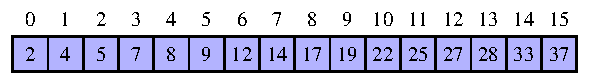
\includegraphics[width=0.7\linewidth]{img/figure-5-4}
\end{figure}

Elemento buscado: $22$.

\medskip

Funcionamento:

\begin{figure}[H]
	\centering
	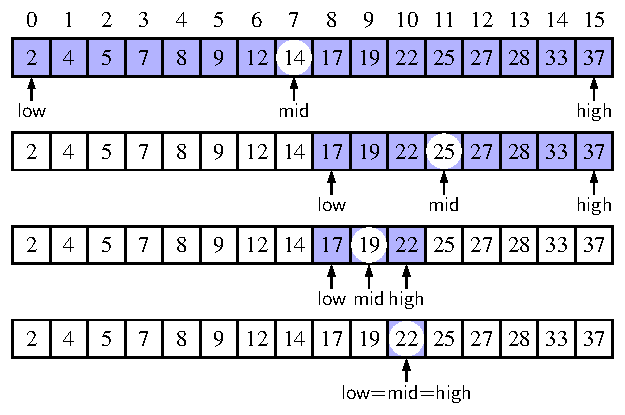
\includegraphics[width=0.7\linewidth]{img/figure-5-5}
\end{figure}

Conclusão:
\begin{itemize}
	\item Encontra o elemento com 4 avaliações ($14$, $25$, $19$ e $22$).
	\item Caso o elemento buscado fosse $23$, na próxima iteração identificaria sua inexistência, pois \texttt{high < low}.
\end{itemize}

\clearpage

Busca binária simples:
\begin{minted}{java}
public class SimpleBinarySearch {
	public int search(int[] array, int value) {
		int start = 0;
		int end = array.length - 1;
		int mid;
		
		do {
			mid = (start + end) / 2;
			if(array[mid] < value)
				start = mid + 1;
			else
				end = mid - 1;	
		} while(array[mid] != value && start <= end);
		
		if(array[mid] == value)
			return mid;
		else
			return -1;
	}
	
	public int search(String[] array, String value) {
		int start = 0;
		int end = array.length - 1;
		int mid;
		
		do {
			mid = (start + end) / 2;
			if(array[mid].compareTo(value) < 0)
				start = mid + 1;
			else
				end = mid - 1;
		} while(array[mid].compareTo(value) != 0 && start <= end);
		
		if(array[mid].compareTo(value) == 0)
			return mid;
		else
			return -1;
	}
}
\end{minted}

\medskip

{\color{redtext}
Comentários:
\begin{itemize}
	\item Veriáveis \texttt{start} e \texttt{end} delimitam a sub-lista de busca (equivalente a \texttt{low} e \texttt{high}).
	\item Enquanto não encontra, atualiza o intervalo de índices e repete o processo.
	\item Quando \texttt{start > end}, finaliza a busca sem sucesso.
\end{itemize}
}

\medskip

Busca binária genérica:
\begin{minted}{java}
public class GenericBinarySearch<E> {
	
	Comparator<E> comp;
	
	public GenericBinarySearch() {
		this(new DefaultComparator<E>());
	}
	
	public GenericBinarySearch(Comparator<E> c) {
		comp = c;
	}
	
	public int indexOf(E[] array, E value) {
		int start = 0;
		int end = array.length - 1;
		int mid;
		
		do {
			mid = (start + end) / 2;
			if(comp.compare(array[mid], value) < 0)
				start = mid + 1;
			else
				end = mid - 1;		
		} while(comp.compare(array[mid], value) != 0 && start <= end);
		
		if(comp.compare(array[mid], value) == 0)
			return mid;
		else
			return -1;
	}
	
	public int indexOf(List<E> array, E value) {
		int start = 0;
		int end = array.size() - 1;
		int mid;
		
		do {
			mid = (start + end) / 2;
			if(comp.compare(array.get(mid), value) < 0)
				start = mid + 1;
			else
				end = mid - 1;	
		} while(comp.compare(array.get(mid), value) != 0 && start <= end);
		
		if(comp.compare(array.get(mid), value) == 0)
			return mid;
		else
			return -1;
	}
}
\end{minted}

\medskip

Busca binária genérica para entradas:
\begin{minted}{java}
public class GenericBinaryEntrySearch<K,V> {
	
	Comparator<K> comp;
	
	public GenericBinaryEntrySearch() {
		this(new DefaultComparator<K>());
	}
	
	public GenericBinaryEntrySearch(Comparator<K> c) {
		comp = c;
	}
	
	public V searchElement(List<Entry<K,V>> array, K key) {
		int start = 0;
		int end = array.size() - 1;
		int mid;
		
		do {
			mid = (start + end) / 2;
			if(comp.compare(array.get(mid).getKey(), key) < 0)
				start = mid + 1;
			else
				end = mid - 1;		
		} while(comp.compare(array.get(mid).getKey(), key) != 0 && start <= end);
		
		if(comp.compare(array.get(mid).getKey(), key) == 0)
			return array.get(mid).getValue();
		else
			return null;
	}
}
\end{minted}

\medskip

{\color{redtext}
	Comentários:
	\begin{itemize}
		\item Veja as aplicações das buscas em diferentes estruturas nas classes \texttt{TestSequentialSearch} e \texttt{TestBinarySearch}.
	\end{itemize}
}

\clearpage

\newtitle{Atividades}

\begin{enumerate}
	\item Desenvolva um software para gerenciar as contas de um banco. Primeiro, armazene os dados em uma estrutura de dados não-ordenada e utilize o algoritmo de busca sequencial para buscar contas. Após isso, implemente uma versão utilizando uma estrutura de dados ordenada, e aplique o algoritmo de busca binária para a pesquisa. Compare o tempo de execução de ambas abordagens para diferentes quantidades de contas armazenadas. Verifique a complexidade empírica dos algoritmos e compare com a complexidade no pior caso.

	\item Implemente uma versão recursiva do algoritmo de busca binária. Em caso de dúvidas, consulte a Seção 5.1.3 de~\cite{GoodrichEtAl2014}.
	
	\item Simule o algoritmo de busca binária para os seguintes casos:
	\begin{enumerate}[a)]
		\item \texttt{x = 15}, \texttt{v = \{15, 27, 33, 46, 51, 63, 71, 82, 90\}}.
		\item \texttt{x = 33}, \texttt{v = \{15, 27, 33, 46, 51, 63, 71, 82, 90\}}.
		\item \texttt{x = 63}, \texttt{v = \{15, 27, 33, 46, 51, 63, 71, 82, 90\}}.
		\item \texttt{x = 81}, \texttt{v = \{15, 27, 33, 46, 51, 63, 71, 82, 90\}}.
		\item \texttt{x = 22}, \texttt{v = \{15, 27, 33, 46, 51, 63, 71, 82, 90\}}.
	\end{enumerate}
	Compare o número de avaliações realizadas com o número de avaliações que uma busca sequencial faria.
	
	\item Quando o vetor está ordenado, a busca sequencial não precisa percorrer toda a lista para saber que o elemento buscado não existe. Ela pode parar quando o elemento analisado for maior que o buscado. Implemente as modificações necessárias para esta estratégia. Qual a complexidade no pior caso do novo algoritmo?
	
	\item Implemente os algoritmos de busca sequencial e binária nas estruturas de dados estudadas em sala de aula.
	
	\item Veja as demonstrações de buscas sequencial e binária disponíveis em \url{https://www.cs.usfca.edu/~galles/visualization/Search.html}. 
\end{enumerate}

\medskip

\newtitle{Referências}
\begingroup
	\footnotesize
	\renewcommand{\chapter}[2]{}%
	\bibliographystyle{apalike}
	\bibliography{../referencias}
\endgroup

\end{document}